\pdfminorversion=4 % for acroread
%\documentclass[aspectratio=169,t,xcolor={usenames,dvipsnames}]{beamer}
\documentclass[aspectratio=169,t,handout,xcolor={usenames,dvipsnames}]{beamer}
\usepackage{../beamerstyle}
\usepackage{dsfont}
\usepackage{bm}
\usepackage[english]{babel}
\usepackage[utf8]{inputenc}
\usepackage{graphicx}
\usepackage{algorithm}
\usepackage[ruled,vlined,algo2e,linesnumbered]{algorithm2e}
%\usepackage[boxed,vlined]{algorithm2e}
\usepackage{hyperref}
\usepackage{booktabs}
\usepackage{mathtools}

\usepackage{amsmath,amssymb}
\usepackage{listings}
\lstset{frame=lines,framesep=3pt,numbers=left,numberblanklines=false,basicstyle=\ttfamily\small}

\usepackage{subfig}
\usepackage{multicol}
%\usepackage{appendixnumberbeamer}
%
\usepackage{tcolorbox}

\usepackage{pgfplots}
\usepackage{tikz}
\usetikzlibrary{trees} 
\usetikzlibrary{shapes.geometric}
\usetikzlibrary{positioning,shapes,shadows,arrows,calc,mindmap}
\usetikzlibrary{positioning,fadings,through}
\usetikzlibrary{decorations.pathreplacing}
\usetikzlibrary{intersections}
\usetikzlibrary{positioning,fit,calc,shadows,backgrounds}
\pgfdeclarelayer{background}
\pgfdeclarelayer{foreground}
\pgfsetlayers{background,main,foreground}
\tikzstyle{activity}=[rectangle, draw=black, rounded corners, text centered, text width=8em]
\tikzstyle{data}=[rectangle, draw=black, text centered, text width=8em]
\tikzstyle{myarrow}=[->, thick, draw=black]

% Define the layers to draw the diagram
\pgfdeclarelayer{background}
\pgfdeclarelayer{foreground}
\pgfsetlayers{background,main,foreground}

%\usepackage{listings}
%\lstset{numbers=left,
%  showstringspaces=false,
%  frame={tb},
%  captionpos=b,
%  lineskip=0pt,
%  basicstyle=\ttfamily,
%%  extendedchars=true,
%  stepnumber=1,
%  numberstyle=\small,
%  xleftmargin=1em,
%  breaklines
%}

 
\definecolor{blue}{RGB}{0, 74, 153}

\usetheme{Boadilla}
%\useinnertheme{rectangles}
\usecolortheme{whale}
\setbeamercolor{alerted text}{fg=blue}
\useoutertheme{infolines}
\setbeamertemplate{navigation symbols}{\vspace{-5pt}} % to lower the logo
\setbeamercolor{date in head/foot}{bg=white} % blue
\setbeamercolor{date in head/foot}{fg=white}
\setbeamercolor{author  in head/foot}{bg=white} %blue
\setbeamercolor{title in head/foot}{bg=white} % blue
\setbeamercolor{title}{fg=white, bg=blue}
\setbeamercolor{block title}{fg=white,bg=blue}
\setbeamercolor{block body}{bg=blue!10}
\setbeamercolor{frametitle}{fg=white, bg=blue}
\setbeamercovered{invisible}

\makeatletter
\setbeamertemplate{footline}
{
  \leavevmode%
  \hbox{%
  \begin{beamercolorbox}[wd=.333333\paperwidth,ht=2.25ex,dp=1ex,center]{author in head/foot}%
%    \usebeamerfont{author in head/foot}\insertshortauthor
  \end{beamercolorbox}%
  \begin{beamercolorbox}[wd=.333333\paperwidth,ht=2.25ex,dp=1ex,center]{title in head/foot}%
    \usebeamerfont{title in head/foot}\insertshorttitle
  \end{beamercolorbox}%
  \begin{beamercolorbox}[wd=.333333\paperwidth,ht=2.25ex,dp=1ex,right]{date in head/foot}%
    \usebeamerfont{date in head/foot}\insertshortdate{}\hspace*{2em}
%    \insertframenumber\hspace*{2ex} 
  \end{beamercolorbox}}%
  \vskip0pt%
}
\makeatother

%\pgfdeclareimage[height=1.2cm]{automl}{images/logos/automl.png}
%\pgfdeclareimage[height=1.2cm]{freiburg}{images/logos/freiburg}

%\logo{\pgfuseimage{freiburg}}

\renewcommand{\comment}[1]{
	\noindent
	%\vspace{0.25cm}
	{\color{red}{\textbf{TODO:} #1}}
	%\vspace{0.25cm}
}
\newcommand{\notefh}[1]{\textcolor{red}{\textbf{FH:} #1}}
\renewcommand{\comment}[1]{}
\newcommand{\hide}[1]{}
\newcommand{\cemph}[2]{\emph{\textcolor{#1}{#2}}}

\newcommand{\lit}[1]{{\footnotesize\color{black!60}[#1]}}

\newcommand{\litw}[1]{{\footnotesize\color{blue!20}[#1]}}


\newcommand{\myframe}[2]{\begin{frame}[c]{#1}#2\end{frame}}
\newcommand{\myframetop}[2]{\begin{frame}{#1}#2\end{frame}}
\newcommand{\myit}[1]{\begin{itemize}#1\end{itemize}}
\newcommand{\myblock}[2]{\begin{block}{#1}#2\end{block}}


\newcommand{\votepurple}[1]{\textcolor{Purple}{$\bigstar$}}
\newcommand{\voteyellow}[1]{\textcolor{Goldenrod}{$\bigstar$}}
\newcommand{\voteblue}[1]{\textcolor{RoyalBlue}{$\bigstar$}}
\newcommand{\votepink}[1]{\textcolor{Pink}{$\bigstar$}}

\newcommand{\diff}{\mathop{}\!\mathrm{d}}
\newcommand{\refstyle}[1]{{\small{\textcolor{gray}{#1}}}}
\newcommand{\hands}[0]{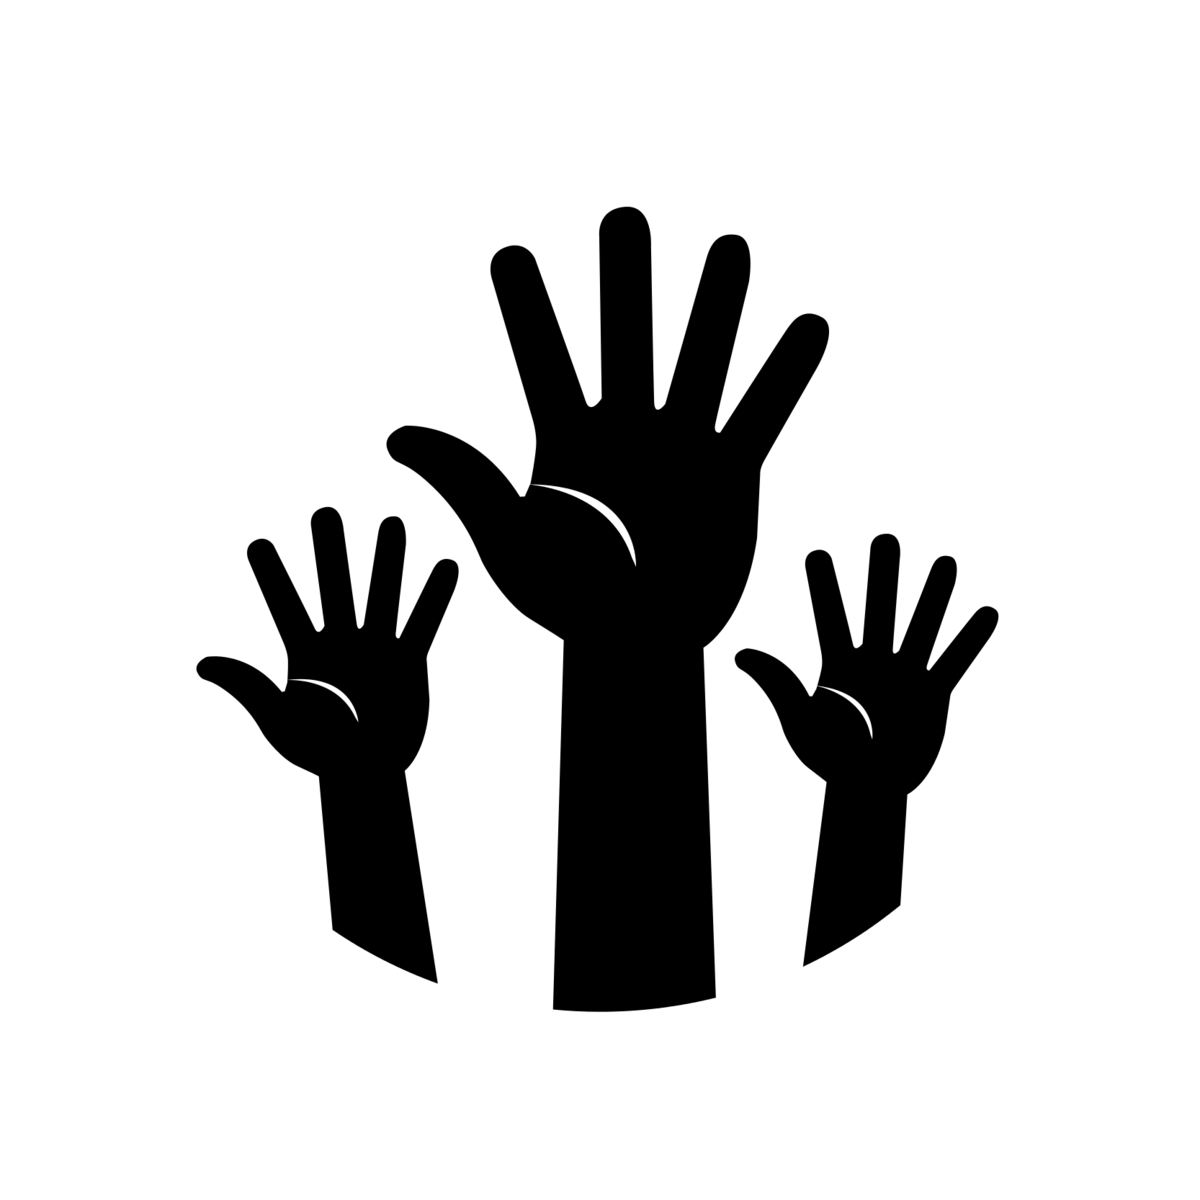
\includegraphics[height=1.5em]{images/hands}}
\newcommand{\transpose}[0]{{\textrm{\tiny{\sf{T}}}}}
\newcommand{\norm}{{\mathcal{N}}}
\newcommand{\cutoff}[0]{\kappa}
\newcommand{\instD}[0]{\dataset}
\newcommand{\insts}[0]{\mathcal{I}}
\newcommand{\inst}[0]{i}
\newcommand{\instI}[1]{i^{(#1)}}

% Iteration specific instance of variable/function/anything
% Introduced in the BO section, but moved up here to make it available within other macros
\newcommand{\iter}[2][\bocount]{{#2}^{(#1)}}

%--------HPO parameter macros-----------

% Parameter Configuration Space
\newcommand{\pcs}[0]{\pmb{\Lambda}}

% ???
\newcommand{\bx}[0]{\conf}

% Parameter Configuration
\newcommand{\conf}[0]{\pmb{\lambda}}

% Final Configuration
\newcommand{\finconf}[0]{\pmb{\hat{\lambda}}}

% Configuration corresponding to a given iteration -- better use \iter!
\newcommand{\confI}[1]{{\conf}^{(#1)}}

% Default Configuration
\newcommand{\defconf}[0]{{\conf}_{\text{def}}}

% Incumbent Configuration
\newcommand{\incumbent}[1][\bocount]{\iter[#1]{\finconf}}

% Optimal Configuration
\newcommand{\optconf}[0]{{\conf}^*}

% Configuration Space
\newcommand{\confs}[0]{\pcs}

%----------------------------------------

%\newcommand{\vlambda}[0]{\bm{\lambda}}
%\newcommand{\vLambda}[0]{\bm{\Lambda}}
\newcommand{\dataset}[0]{\mathcal{D}}
\newcommand{\datasets}[0]{\mathbf{D}}
\newcommand{\loss}[0]{L}
\newcommand{\risk}{\mathcal{R}}
\newcommand{\riske}{\mathcal{R}_{\text{emp}}}
\newcommand{\cost}[0]{c}
\newcommand{\costI}[1]{c^{(#1)}}

% Gaussian Process
\newcommand{\gp}{\mathcal{G}}
% Family of Objective Functions
\newcommand{\objF}{F}

%---------------BO Macros------------------

% BO loop counter
\newcommand{\bocount}{t}
% BO loop counter max, the counter runs from 1 to this value
\newcommand{\bobudget}{T}
% BO loop observation
\newcommand{\obs}[1][\conf]{\cost({#1})}
% BO loop observation space
\newcommand{\obsspace}{\mathcal{Y}}
% BO loop next observation
\newcommand{\bonextobs}{\obs[\iter{\conf}]}
% Acquisition Function, no args
\newcommand{\acq}{u}
% Standard Normal PDF
\newcommand{\pdf}{\phi}
% Standard Normal CDF
\newcommand{\cdf}{\Phi}
% Mean
\newcommand{\mean}{\mu}
% Standard Deviation
\newcommand{\stddev}{\sigma}
% Variance
\newcommand{\variance}{\sigma^2}
% Noise
\newcommand{\noise}{\nu}
% BO loop next selected sample
\newcommand{\bonextsample}{\confI{\bocount}}

% Single hyperparameter
\newcommand{\hyperparam}{\lambda}

% Single hyperparameter within a hyperparameter configuration
\newcommand{\hyperparami}[1][i]{{\hyperparam}_#1}

% Full definition of final configuration
\newcommand{\finconffull}{\incumbent[\bobudget]}

% Dataset
\newcommand{\datasetHPO}{{\dataset}_{HPO}}

% Dataset definition
\newcommand{\datasetHPOdef}{{\langle \bonextsample,\,\bonextobs \rangle}_{\bocount=1}^{\bobudget}}

% Double Display Fraction, forces large displays for everything in numerator and denominator
\newcommand\ddfrac[2]{\frac{\displaystyle #1}{\displaystyle #2}}

% Conditional Probability "Given That" Relation, source:https://tex.stackexchange.com/a/141685/205886
\newcommand\given[1][]{\:#1\vert\:}

% Expectation as a math operator
\DeclareMathOperator*{\E}{\mathbb{E}}

% Citation 
\newcommand{\source}[1]{
    \begin{flushright}
    	Source: \lit{#1}
    \end{flushright}
}
%-------------------------------------------

%Real numbers set
\newcommand{\realnum}{\mathbb{R}}
%Configuration space - do not use
%\newcommand{\configspace}{\Theta}
%Instances - do not use
%\newcommand{\instances}{\mathcal{I}}
%Expected value
\newcommand{\expectation}{\mathbb{E}}
%Kernel
\newcommand{\kernel}{\kappa}
%Constraint function
\newcommand{\constraintf}{c}
%Normal distribution
\newcommand{\normaldist}{\mathcal{N}}

% \renewcommand{\vec}[1]{\mathbf{#1}}
\newcommand{\hist}[0]{\dataset_{\text{Hist}}}
\newcommand{\param}[0]{p}
\newcommand{\algo}[0]{\mathcal{A}}
\newcommand{\algos}[0]{\mathbf{A}}
%\newcommand{\nn}[0]{N}
\newcommand{\feats}[0]{\mathcal{X}_{\text{meta}}}
\newcommand{\feat}[0]{\x_{\text{meta}}}
%\newcommand{\cluster}[0]{\vec{h}}
%\newcommand{\clusters}[0]{\vec{H}}
\newcommand{\perf}[0]{\mathbb{R}}
%\newcommand{\surro}[0]{\mathcal{S}}
\newcommand{\surro}[0]{\hat{\cost}}
\newcommand{\func}[0]{f}
\newcommand{\epm}[0]{\surro}
\newcommand{\portfolio}[0]{\mathbf{P}}
\newcommand{\schedule}[0]{\mathcal{S}}

% Machine Learning
\newcommand{\mdata}[0]{\dataset_{\text{meta}}}
\newcommand{\datasettrain}[0]{\dataset_{\text{train}}}
\newcommand{\datasetval}[0]{\dataset_{\text{val}}}
\newcommand{\datasettest}[0]{\dataset_{\text{test}}}
\newcommand{\x}[0]{\mathbf{x}}
\newcommand{\y}[0]{y}
\newcommand{\xI}[1]{\mathbf{x}^{(#1)}}
\newcommand{\yI}[1]{y^{(#1)}}
\newcommand{\fx}{f(\mathbf{x})}  % f(x), continuous prediction function
\newcommand{\Hspace}{\mathcal{H}} % hypothesis space where f is from
\newcommand{\fh}{\hat{f}}       % f hat, estimated prediction function

% Deep Learning
\newcommand{\weights}[0]{\theta}
\newcommand{\metaweights}[0]{\phi}


% reinforcement learning
\newcommand{\policies}[0]{\mathbf{\Pi}}
\newcommand{\policy}[0]{\pi}
\newcommand{\actionRL}[0]{a}
\newcommand{\stateRL}[0]{s}
\newcommand{\statesRL}[0]{\mathcal{S}}
\newcommand{\rewardRL}[0]{r}
\newcommand{\rewardfuncRL}[0]{\mathcal{R}}

\RestyleAlgo{algoruled}
\DontPrintSemicolon
\LinesNumbered
\SetAlgoVlined
\SetFuncSty{textsc}

\SetKwInOut{Input}{Input}
\SetKwInOut{Output}{Output}
\SetKw{Return}{return}

%\newcommand{\changed}[1]{{\color{red}#1}}

%\newcommand{\citeN}[1]{\citeauthor{#1}~(\citeyear{#1})}

\renewcommand{\vec}[1]{\mathbf{#1}}
\DeclareMathOperator*{\argmin}{arg\,min}
\DeclareMathOperator*{\argmax}{arg\,max}

%\newcommand{\aqme}{\textit{AQME}}
%\newcommand{\aslib}{\textit{ASlib}}
%\newcommand{\llama}{\textit{LLAMA}}
%\newcommand{\satzilla}{\textit{SATzilla}}
%\newcommand{\satzillaY}[1]{\textit{SATzilla'{#1}}}
%\newcommand{\snnap}{\textit{SNNAP}}
%\newcommand{\claspfolioTwo}{\textit{claspfolio~2}}
%\newcommand{\flexfolio}{\textit{FlexFolio}}
%\newcommand{\claspfolioOne}{\textit{claspfolio~1}}
%\newcommand{\isac}{\textit{ISAC}}
%\newcommand{\eisac}{\textit{EISAC}}
%\newcommand{\sss}{\textit{3S}}
%\newcommand{\sunny}{\textit{Sunny}}
%\newcommand{\ssspar}{\textit{3Spar}}
%\newcommand{\cshc}{\textit{CSHC}}
%\newcommand{\cshcpar}{\textit{CSHCpar}}
%\newcommand{\measp}{\textit{ME-ASP}}
%\newcommand{\aspeed}{\textit{aspeed}}
%\newcommand{\autofolio}{\textit{AutoFolio}}
%\newcommand{\cedalion}{\textit{Cedalion}}
\newcommand{\fanova}{\textit{fANOVA}}
\newcommand{\sbs}{\textit{SB}}
\newcommand{\oracle}{\textit{VBS}}

% like approaches
\newcommand{\claspfoliolike}[1]{\texttt{claspfolio-#1-like}}
\newcommand{\satzillalike}[1]{\texttt{SATzilla'#1-like}}
\newcommand{\isaclike}{\texttt{ISAC-like}}
\newcommand{\ssslike}{\texttt{3S-like}}
\newcommand{\measplike}{\texttt{ME-ASP-like}}

\newcommand{\irace}{\textit{I/F-race}}
\newcommand{\gga}{\textit{GGA}}
\newcommand{\smac}{\textit{SMAC}}
\newcommand{\paramils}{\textit{ParamILS}}
\newcommand{\spearmint}{\textit{Spearmint}}
\newcommand{\tpe}{\textit{TPE}}


\usepackage{pifont}
\newcommand{\itarrow}{\mbox{\Pisymbol{pzd}{229}}}
\newcommand{\ithook}{\mbox{\Pisymbol{pzd}{52}}}
\newcommand{\itcross}{\mbox{\Pisymbol{pzd}{56}}}
\newcommand{\ithand}{\mbox{\raisebox{-1pt}{\Pisymbol{pzd}{43}}}}

%\DeclareMathOperator*{\argmax}{arg\,max}

\newcommand{\ie}{{\it{}i.e.\/}}
\newcommand{\eg}{{\it{}e.g.\/}}
\newcommand{\cf}{{\it{}cf.\/}}
\newcommand{\wrt}{\mbox{w.r.t.}}
\newcommand{\vs}{{\it{}vs\/}}
\newcommand{\vsp}{{\it{}vs\/}}
\newcommand{\etc}{{\copyedit{etc.}}}
\newcommand{\etal}{{\it{}et al.\/}}

\newcommand{\pscProc}{{\bf procedure}}
\newcommand{\pscBegin}{{\bf begin}}
\newcommand{\pscEnd}{{\bf end}}
\newcommand{\pscEndIf}{{\bf endif}}
\newcommand{\pscFor}{{\bf for}}
\newcommand{\pscEach}{{\bf each}}
\newcommand{\pscThen}{{\bf then}}
\newcommand{\pscElse}{{\bf else}}
\newcommand{\pscWhile}{{\bf while}}
\newcommand{\pscIf}{{\bf if}}
\newcommand{\pscRepeat}{{\bf repeat}}
\newcommand{\pscUntil}{{\bf until}}
\newcommand{\pscWithProb}{{\bf with probability}}
\newcommand{\pscOtherwise}{{\bf otherwise}}
\newcommand{\pscDo}{{\bf do}}
\newcommand{\pscTo}{{\bf to}}
\newcommand{\pscOr}{{\bf or}}
\newcommand{\pscAnd}{{\bf and}}
\newcommand{\pscNot}{{\bf not}}
\newcommand{\pscFalse}{{\bf false}}
\newcommand{\pscEachElOf}{{\bf each element of}}
\newcommand{\pscReturn}{{\bf return}}

%\newcommand{\param}[1]{{\sl{}#1}}
\newcommand{\var}[1]{{\it{}#1}}
\newcommand{\cond}[1]{{\sf{}#1}}
%\newcommand{\state}[1]{{\sf{}#1}}
%\newcommand{\func}[1]{{\sl{}#1}}
\newcommand{\set}[1]{{\Bbb #1}}
%\newcommand{\inst}[1]{{\tt{}#1}}
\newcommand{\myurl}[1]{{\small\sf #1}}

\newcommand{\Nats}{{\Bbb N}}
\newcommand{\Reals}{{\Bbb R}}
\newcommand{\extset}[2]{\{#1 \; | \; #2\}}

\newcommand{\vbar}{$\,\;|$\hspace*{-1em}\raisebox{-0.3mm}{$\,\;\;|$}}
\newcommand{\vendbar}{\raisebox{+0.4mm}{$\,\;|$}}
\newcommand{\vend}{$\,\:\lfloor$}


\newcommand{\goleft}[2][.7]{\parbox[t]{#1\linewidth}{\strut\raggedright #2\strut}}
\newcommand{\rightimage}[2][.3]{\mbox{}\hfill\raisebox{1em-\height}[0pt][0pt]{\includegraphics[width=#1\linewidth]{#2}}\vspace*{-\baselineskip}}





\title{Speedup Techniques for Hyperparameter Optimization}
\subtitle{Overview}
\author[Frank Hutter]{Bernd Bischl \and \underline{Frank Hutter} \and Lars Kotthoff\newline \and Marius Lindauer \and Joaquin Vanschoren}
\institute{}
\date{}



\begin{document}
\maketitle

%-------------------------------------------------
\begin{frame}{Beyond Black-box Optimization}
\medskip
Recall general blackbox optimization:\\
        \bigskip
        \begin{center}
        \scalebox{0.7}{\hspace*{1.0cm}
        \newcommand{\myblackbox}{\fcolorbox{black}{black}{
    \minipage[t]{\dimexpr0.111\linewidth-2\fboxsep-2\fboxrule\relax}
        ~~~\\
        ~~~\\
        ~~~\\
    \endminipage}}
    
    
    	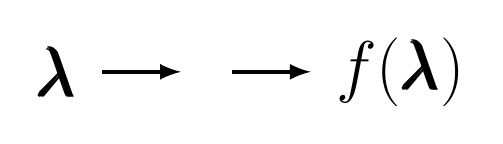
\begin{tikzpicture}
\tikzstyle{every node}=[draw,fill=white,minimum width=0cm,thin]
\tikzstyle{every path}=[-latex,ultra thick]
\node (A) [draw=white]{{\Huge{$\conf$}}};
\node (B) [right=14mm of A,draw=white] {\myblackbox{}};
\node (C) [right=14mm of B,draw=white] {{\Huge{$f(\conf)$}}};
%\node (D) [below=7mm of B, align=center, fill=black!10] {\large{Bayesian}\\\large{optimization}};

\draw ($(A.east)+(0.2,0.0)$) -- ($(B.west)+(-0.2,0.0)$);
\draw ($(B.east)+(0.2,0.0)$) -- ($(C.west)+(-0.2,0.0)$);
%\draw ($(C.south)+(0.0,-0.2)$) -| ++(0.0,0.0) |- ($(D.east)+(0.2,0.0)$);
%\draw ($(D.west)+(-0.2,0.0)$) |- ++(0.0,0.0) -| ($(A.south)+(0.0,-0.2)$);
\end{tikzpicture}
}\\
        \bigskip
         Only mode of interaction with $f$: querying $f$'s value at a given $\conf$
        
\pause
        \bigskip
        \bigskip
        \huge{\textcolor{red}{Too slow for tuning expensive models}}
        
        \end{center}
\vspace*{-6cm}
\begin{center}
\scalebox{15}{\color{Red}{$\bm{\times}$}}
\end{center}    
    
\end{frame}
%-------------------------------------------------

%-------------------------------------------------
%  \begin{frame}{Outline}
%    \bigskip
%    \vfill
%    \tableofcontents
%  \end{frame}
%-------------------------------------------------


\myframetop{Methods for Going Beyond Blackbox Bayesian Optimization}{

	\begin{columns}
	\column{0.0\textwidth}
	\column{0.8\textwidth}
	
		\vspace*{-0.4cm}
	    \myit{
			\onslide<1->{
				\item \alert{Sum of little black boxes}
	        	\myit{
		        	\item Each little black box is fast but only yields a noisy estimate \\
		        	\item SMAC \lit{\href{https://ml.informatik.uni-freiburg.de/papers/11-LION5-SMAC.pdf}{Hutter et al. 2011}} directly solves $\argmin_{\conf\in\confs} \sum_{i=1}^N \cost(\conf,i)$ 	        	
		        	\item Auto-WEKA \lit{\href{https://dl.acm.org/doi/10.1145/2487575.2487629}{Thornton et al, 2013}} used this to optimize 10-fold cross-validation performance
		        }
			}\onslide<2->{
				\bigskip
				\item \alert{Meta-learning across problems / datasets}
				\bigskip
				\bigskip
			}\onslide<3->{
			    \item \alert{Multi-fidelity optimization} 
		   		\bigskip
		   		\bigskip
		   		\medskip
		    }\onslide<4->{
			    \item \alert{Graybox optimization / learning curve prediction} 
		    }
	    }
	\column{0.2\textwidth}
		\vspace*{-0.4cm}
		\onslide<1->{
			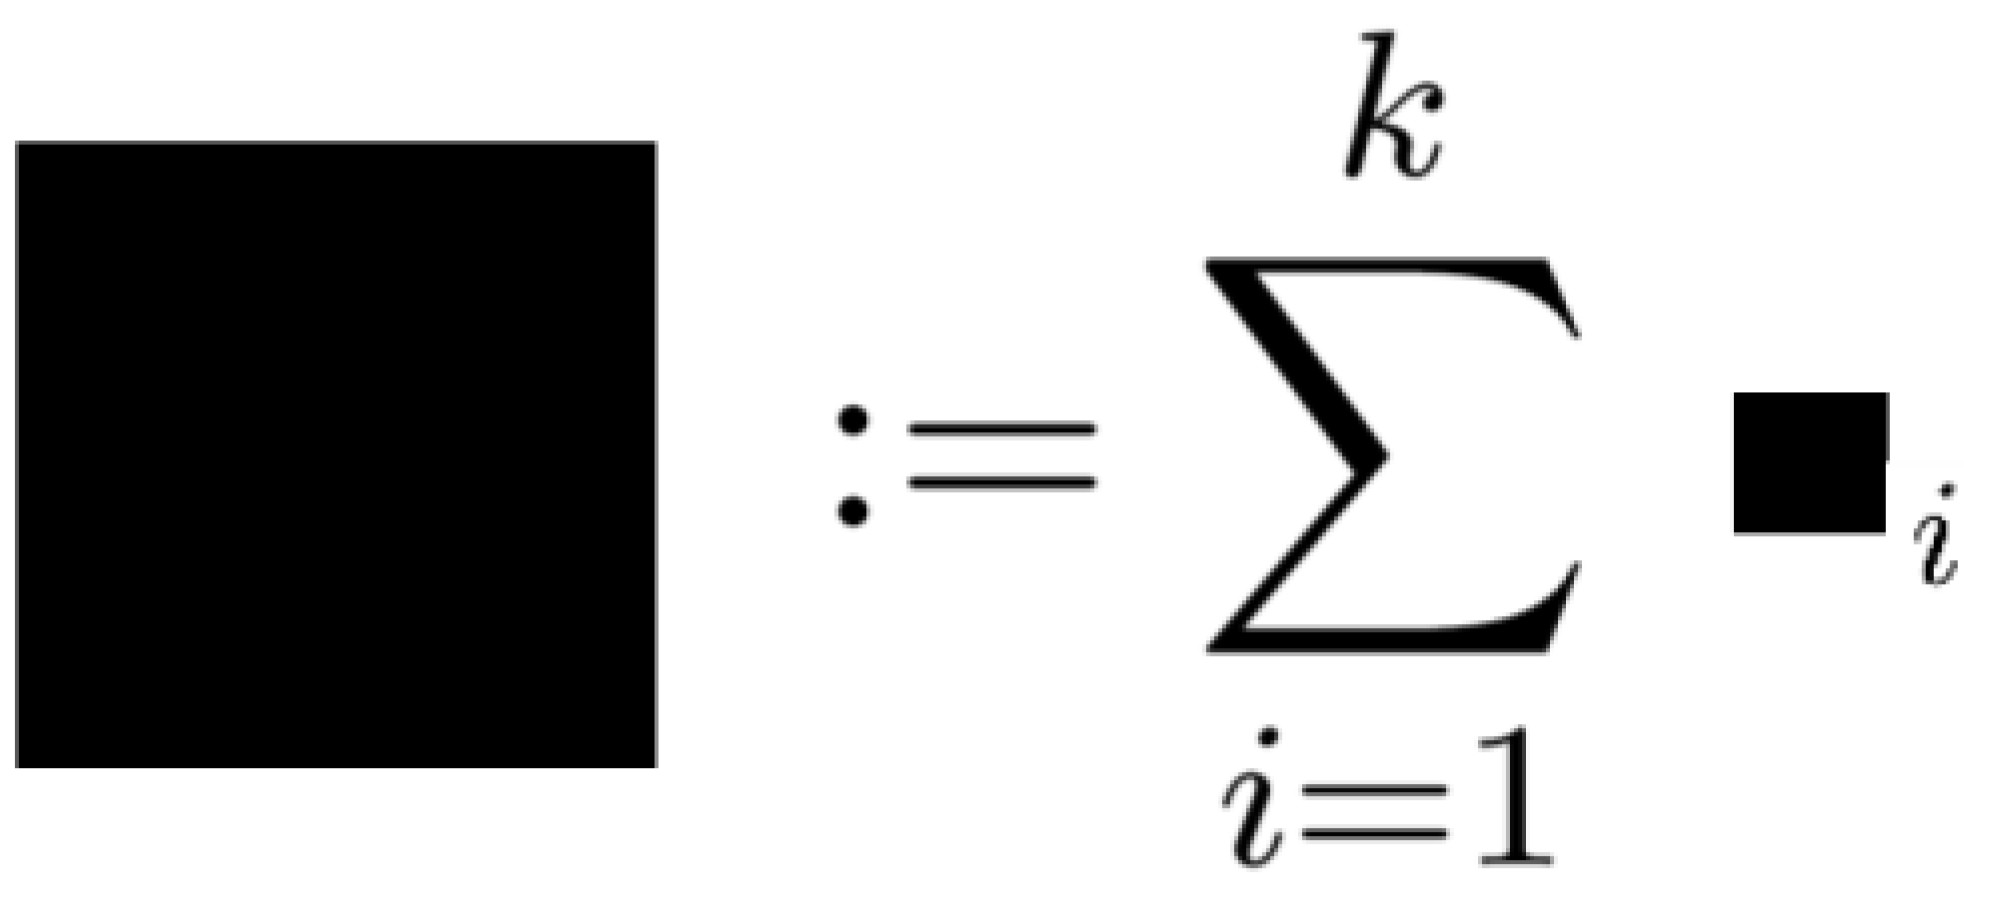
\includegraphics[width=\linewidth, keepaspectratio=true]{images/intro/Sum_of_little_blackboxes.png}
		}\onslide<2->{
			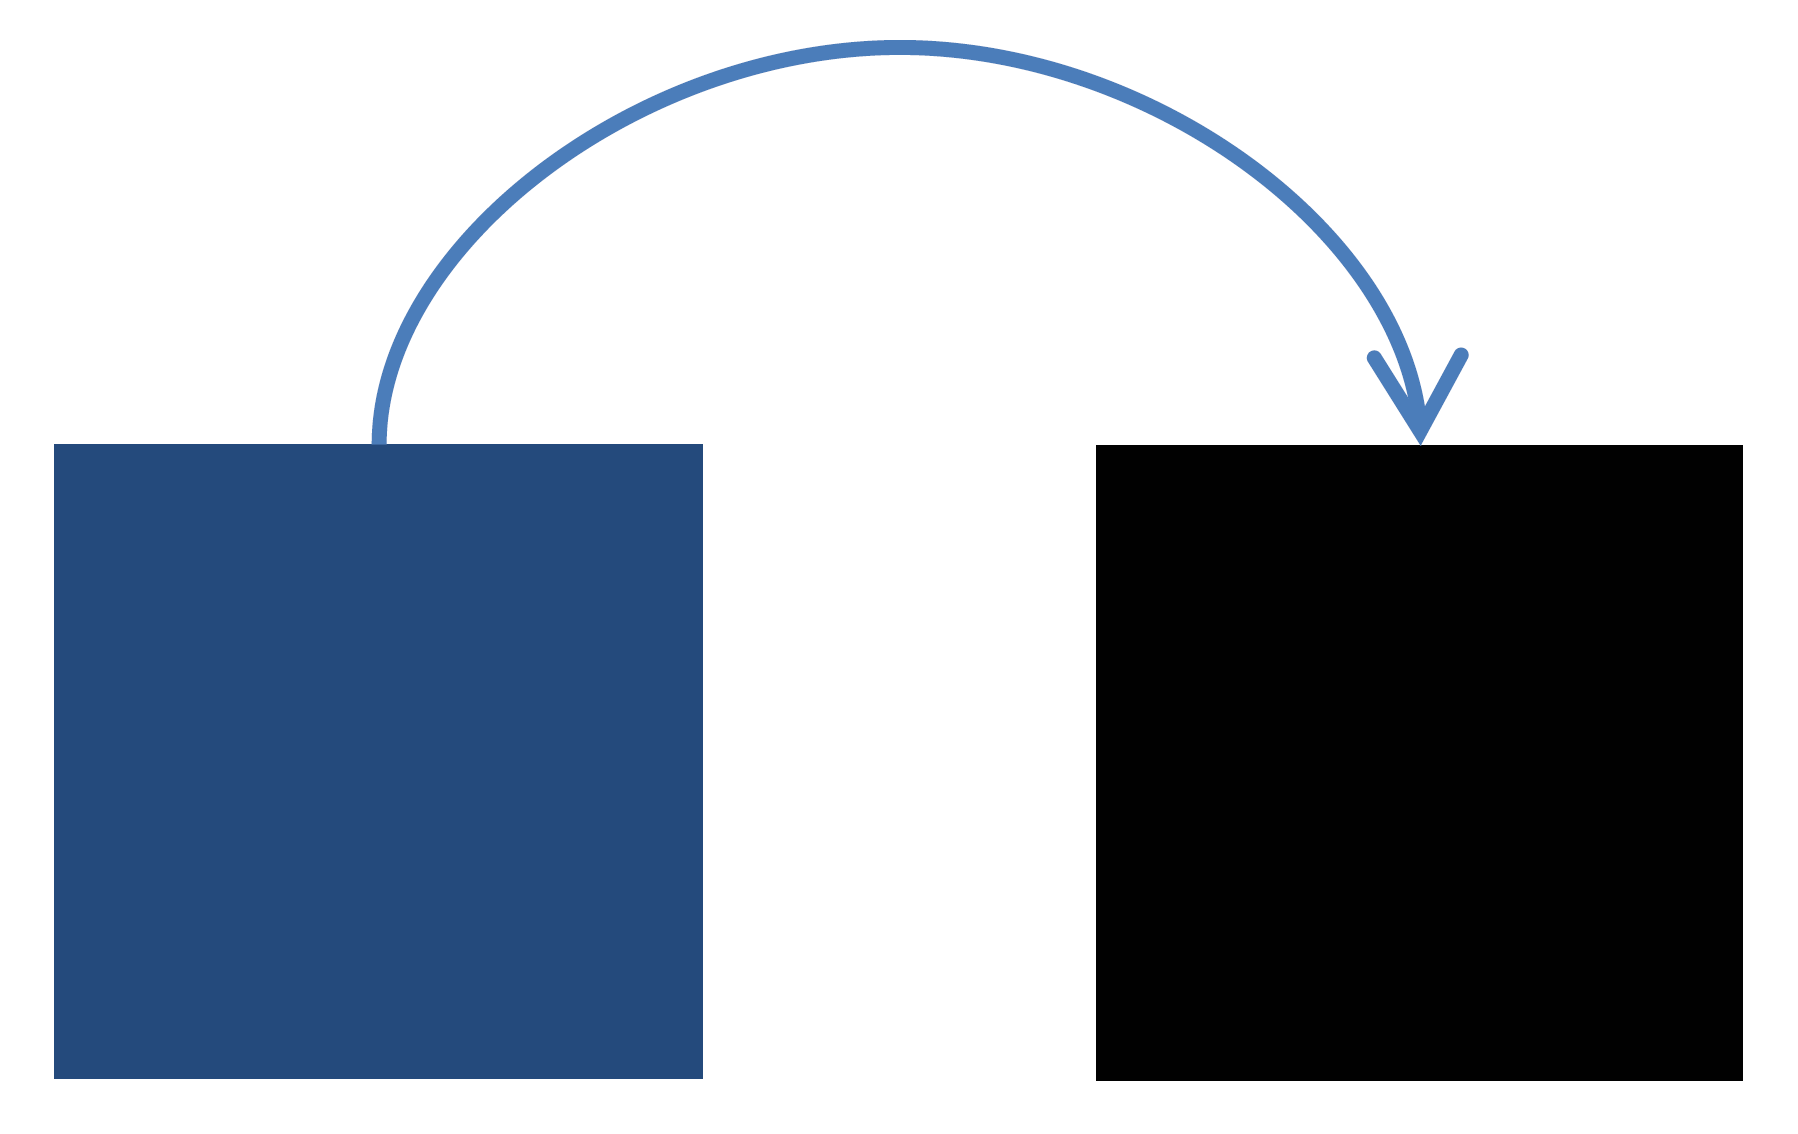
\includegraphics[width=\linewidth, keepaspectratio=true]{images/intro/meta-learning.png}
			\smallskip
		}\onslide<3->{
%			\smallskip~
			\smallskip
			\vspace*{-0.3cm}
			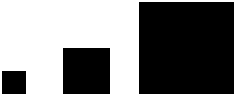
\includegraphics[width=\linewidth, keepaspectratio=true]{images/intro/black_blocks.png}
			\smallskip
		}\onslide<4->{
%			\vspace*{0.5cm}~
			\hspace*{-2.5cm}~
			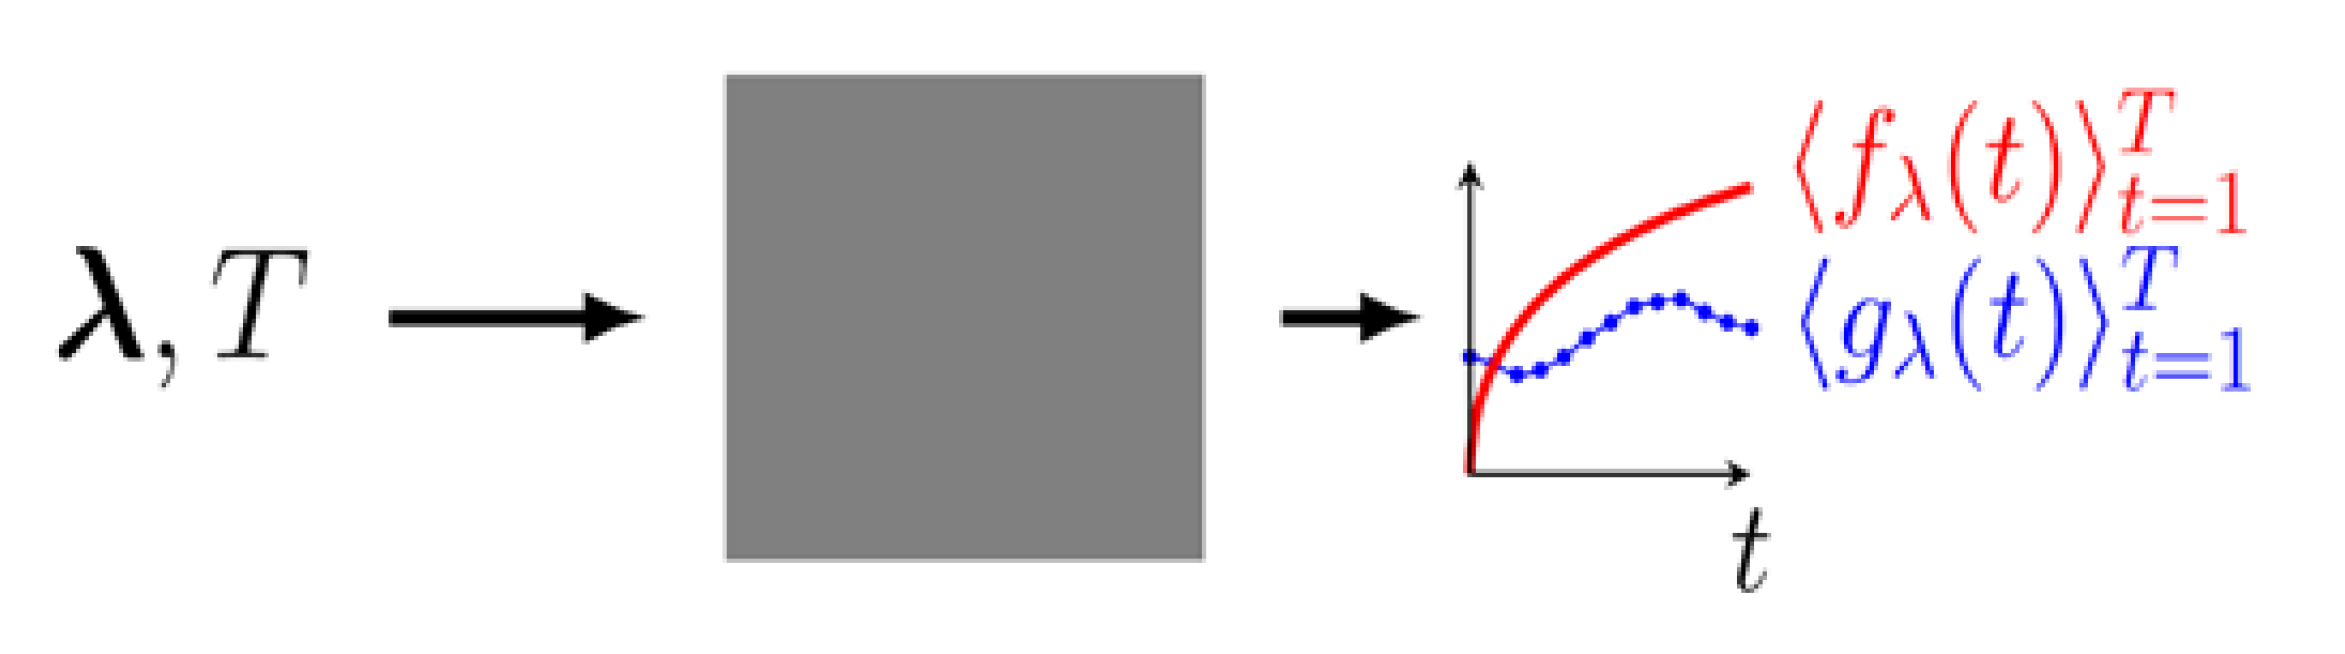
\includegraphics[width=1.8\linewidth, keepaspectratio=true]{images/intro/graybox_optimization.png}
		}   
		\end{columns}
	
}



%-----------------------------------------------------------------------

\begin{frame}[c]{Learning Goals of this Lecture}
\framesubtitle{After this lecture, students can ...}

\begin{itemize}
    \item Describe many different ways of using \alert{meta-learning} to speed up HPO
    \item Explain the concept of \alert{multi-fidelity} optimization to speed up HPO
    \item Explain the \alert{Successive Halving} and \alert{Hyperband} algorithms 
    \item Explain how to combine Bayesian optimization and Hyperband in \alert{BOHB}
    \item Describe how to \alert{exploit multiple fidelities in Bayesian optimization} 
    \item Discuss several ways of predicting \alert{learning curves}
    \item Discuss \alert{success stories} of speeding up Bayesian optimization
%    \item Describe \alert{gradient descent} approaches for HPO
\end{itemize}
\end{frame}

%-----------------------------------------------------------------------











%-------------------------------------------------
\iffalse


%-------------------------------------------------
\begin{frame}{Recall: Black-box optimization}

\begin{figure}
    \centering
    


\tikzset{every picture/.style={line width=0.75pt}} %set default line width to 0.75pt        

\begin{tikzpicture}[x=0.70pt,y=0.70pt,yscale=-1,xscale=1]
%uncomment if require: \path (0,300); %set diagram left start at 0, and has height of 300

%Straight Lines [id:da5075678478287002] 
\draw    (74.5,104) -- (218.5,104) ;
\draw [shift={(220.5,104)}, rotate = 180] [color={rgb, 255:red, 0; green, 0; blue, 0 }  ][line width=0.75]    (10.93,-3.29) .. controls (6.95,-1.4) and (3.31,-0.3) .. (0,0) .. controls (3.31,0.3) and (6.95,1.4) .. (10.93,3.29)   ;
%Shape: Square [id:dp6368535923226633] 
\draw  [fill={rgb, 255:red, 0; green, 25; blue, 255 }  ,fill opacity=1 ] (14,79) -- (64,79) -- (64,129) -- (14,129) -- cycle ;
%Shape: Square [id:dp8011400143211207] 
\draw  [fill={rgb, 255:red, 0; green, 25; blue, 255 }  ,fill opacity=1 ] (561,79) -- (611,79) -- (611,129) -- (561,129) -- cycle ;
%Straight Lines [id:da6772752516220095] 
\draw    (401.5,101) -- (540.5,101.99) ;
\draw [shift={(542.5,102)}, rotate = 180.41] [color={rgb, 255:red, 0; green, 0; blue, 0 }  ][line width=0.75]    (10.93,-3.29) .. controls (6.95,-1.4) and (3.31,-0.3) .. (0,0) .. controls (3.31,0.3) and (6.95,1.4) .. (10.93,3.29)   ;
%Straight Lines [id:da7102938160527976] 
\draw    (39.5,242) -- (39.01,143) ;
\draw [shift={(39,141)}, rotate = 449.72] [color={rgb, 255:red, 0; green, 0; blue, 0 }  ][line width=0.75]    (10.93,-3.29) .. controls (6.95,-1.4) and (3.31,-0.3) .. (0,0) .. controls (3.31,0.3) and (6.95,1.4) .. (10.93,3.29)   ;
%Straight Lines [id:da5275375794470956] 
\draw    (39.5,242) -- (123.5,242) ;
%Straight Lines [id:da11206880859629287] 
\draw    (123.5,242) -- (586.5,242) ;
%Straight Lines [id:da8957848321230528] 
\draw    (586.5,135) -- (586.5,242) ;
%Image [id:dp5678753924043267] 
\draw (313.5,101.5) node  {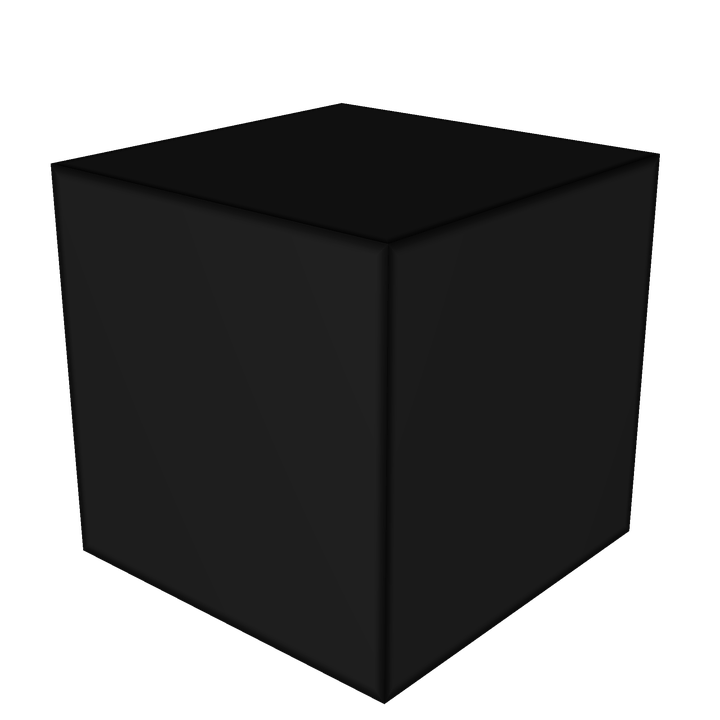
\includegraphics[width=106.5pt,height=104.25pt]{w07_hpo_grey_box/images/intro/black_box.png}};

% Text Node
\draw (284,106.5) node   [align=left] { \textcolor[rgb]{1,1,1}{{\Huge ?}}};
% Text Node
\draw (39,104) node   [align=left] {\textcolor[rgb]{1,1,1}{X}};
% Text Node
\draw (586,102) node   [align=left] {\textcolor[rgb]{1,1,1}{f(X)}};
% Text Node
\draw (317,28) node   [align=left] {Objective function};
% Text Node
\draw (309,254) node   [align=left] {Only interaction: Query of function at $\displaystyle \conf$ to obtain $\displaystyle \cost(\conf)$};


\end{tikzpicture}

\end{figure}
\fhpause
\begin{itemize}
    \item Can we do better?
\end{itemize}
%\source{\lit{\href{https://slideslive.com/38917532/greybox-bayesian-optimization-for-automl}{Peter Frazier: Grey-box Bayesian Optimization for AutoML}}}
    
    \textcolor{red}{FH: can you please create this figure yourself, using the same picture for black box and looking inside the black box, except that for ``looking inside'' the lid is open. For one (not necessarily optimal) way to do this in tikz, see: http://www.texample.net/tikz/examples/annotated-3d-box/}
    
\end{frame}
%-------------------------------------------------




%\section{Introduction to grey-box approaches}
%-------------------------------------------------
%-------------------------------------------------
\begin{frame}{Recall: Black-box optimization}
\begin{figure}
    \centering
    


\tikzset{every picture/.style={line width=0.75pt}} %set default line width to 0.75pt        

\begin{tikzpicture}[x=0.70pt,y=0.70pt,yscale=-1,xscale=1]
%uncomment if require: \path (0,300); %set diagram left start at 0, and has height of 300

%Straight Lines [id:da5075678478287002] 
\draw    (74.5,104) -- (218.5,104) ;
\draw [shift={(220.5,104)}, rotate = 180] [color={rgb, 255:red, 0; green, 0; blue, 0 }  ][line width=0.75]    (10.93,-3.29) .. controls (6.95,-1.4) and (3.31,-0.3) .. (0,0) .. controls (3.31,0.3) and (6.95,1.4) .. (10.93,3.29)   ;
%Shape: Square [id:dp6368535923226633] 
\draw  [fill={rgb, 255:red, 0; green, 25; blue, 255 }  ,fill opacity=1 ] (14,79) -- (64,79) -- (64,129) -- (14,129) -- cycle ;
%Shape: Square [id:dp8011400143211207] 
\draw  [fill={rgb, 255:red, 0; green, 25; blue, 255 }  ,fill opacity=1 ] (561,79) -- (611,79) -- (611,129) -- (561,129) -- cycle ;
%Straight Lines [id:da6772752516220095] 
\draw    (401.5,101) -- (540.5,101.99) ;
\draw [shift={(542.5,102)}, rotate = 180.41] [color={rgb, 255:red, 0; green, 0; blue, 0 }  ][line width=0.75]    (10.93,-3.29) .. controls (6.95,-1.4) and (3.31,-0.3) .. (0,0) .. controls (3.31,0.3) and (6.95,1.4) .. (10.93,3.29)   ;
%Straight Lines [id:da7102938160527976] 
\draw    (39.5,242) -- (39.01,143) ;
\draw [shift={(39,141)}, rotate = 449.72] [color={rgb, 255:red, 0; green, 0; blue, 0 }  ][line width=0.75]    (10.93,-3.29) .. controls (6.95,-1.4) and (3.31,-0.3) .. (0,0) .. controls (3.31,0.3) and (6.95,1.4) .. (10.93,3.29)   ;
%Straight Lines [id:da5275375794470956] 
\draw    (39.5,242) -- (123.5,242) ;
%Straight Lines [id:da11206880859629287] 
\draw    (123.5,242) -- (586.5,242) ;
%Straight Lines [id:da8957848321230528] 
\draw    (586.5,135) -- (586.5,242) ;
%Image [id:dp5678753924043267] 
\draw (313.5,101.5) node  {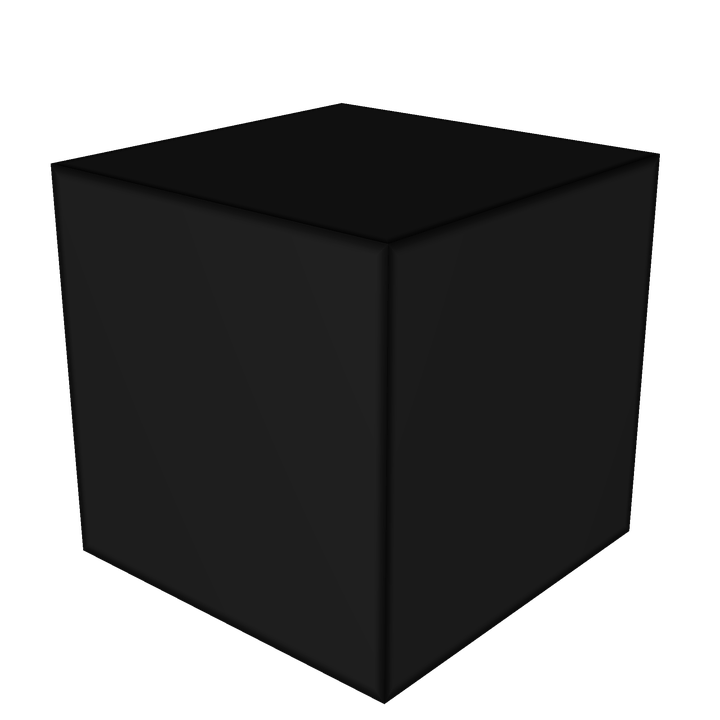
\includegraphics[width=106.5pt,height=104.25pt]{w07_hpo_grey_box/images/intro/black_box.png}};

% Text Node
\draw (284,106.5) node   [align=left] { \textcolor[rgb]{1,1,1}{{\Huge ?}}};
% Text Node
\draw (39,104) node   [align=left] {\textcolor[rgb]{1,1,1}{X}};
% Text Node
\draw (586,102) node   [align=left] {\textcolor[rgb]{1,1,1}{f(X)}};
% Text Node
\draw (317,28) node   [align=left] {Objective function};
% Text Node
\draw (309,254) node   [align=left] {Only interaction: Query of function at $\displaystyle \conf$ to obtain $\displaystyle \cost(\conf)$};


\end{tikzpicture}

\end{figure}
\fhpause
\begin{itemize}
    \item Can we do better?
\end{itemize}
%\source{\lit{\href{https://slideslive.com/38917532/greybox-bayesian-optimization-for-automl}{Peter Frazier: Grey-box Bayesian Optimization for AutoML}}}
    
    \textcolor{red}{FH: can you please create this figure yourself, using the same picture for black box and looking inside the black box, except that for ``looking inside'' the lid is open. For one (not necessarily optimal) way to do this in tikz, see: http://www.texample.net/tikz/examples/annotated-3d-box/}
    
\end{frame}
%-------------------------------------------------
%-------------------------------------------------
\begin{frame}{Looking inside the box}
\begin{figure}
    \centering
    


\tikzset{every picture/.style={line width=0.75pt}} %set default line width to 0.75pt        

\begin{tikzpicture}[x=0.70pt,y=0.70pt,yscale=-1,xscale=1]
%uncomment if require: \path (0,300); %set diagram left start at 0, and has height of 300

%Straight Lines [id:da5075678478287002] 
\draw    (74.5,104) -- (218.5,104) ;
\draw [shift={(220.5,104)}, rotate = 180] [color={rgb, 255:red, 0; green, 0; blue, 0 }  ][line width=0.75]    (10.93,-3.29) .. controls (6.95,-1.4) and (3.31,-0.3) .. (0,0) .. controls (3.31,0.3) and (6.95,1.4) .. (10.93,3.29)   ;
%Shape: Square [id:dp6368535923226633] 
\draw  [fill={rgb, 255:red, 0; green, 25; blue, 255 }  ,fill opacity=1 ] (14,79) -- (64,79) -- (64,129) -- (14,129) -- cycle ;
%Shape: Square [id:dp8011400143211207] 
\draw  [fill={rgb, 255:red, 0; green, 25; blue, 255 }  ,fill opacity=1 ] (561,79) -- (611,79) -- (611,129) -- (561,129) -- cycle ;
%Straight Lines [id:da6772752516220095] 
\draw    (401.5,101) -- (540.5,101.99) ;
\draw [shift={(542.5,102)}, rotate = 180.41] [color={rgb, 255:red, 0; green, 0; blue, 0 }  ][line width=0.75]    (10.93,-3.29) .. controls (6.95,-1.4) and (3.31,-0.3) .. (0,0) .. controls (3.31,0.3) and (6.95,1.4) .. (10.93,3.29)   ;
%Straight Lines [id:da7102938160527976] 
\draw    (39.5,242) -- (39.01,143) ;
\draw [shift={(39,141)}, rotate = 449.72] [color={rgb, 255:red, 0; green, 0; blue, 0 }  ][line width=0.75]    (10.93,-3.29) .. controls (6.95,-1.4) and (3.31,-0.3) .. (0,0) .. controls (3.31,0.3) and (6.95,1.4) .. (10.93,3.29)   ;
%Straight Lines [id:da5275375794470956] 
\draw    (39.5,242) -- (123.5,242) ;
%Straight Lines [id:da11206880859629287] 
\draw    (123.5,242) -- (586.5,242) ;
%Straight Lines [id:da8957848321230528] 
\draw    (586.5,135) -- (586.5,242) ;
%Image [id:dp9410017568713034] 
\draw (307.5,95) node  {
\includegraphics[width=94.5pt,height=76.5pt]{w07_hpo_grey_box/images/intro/opened_box.png}};
%Straight Lines [id:da7498039648909043] 
\draw    (264,72) -- (222.18,45.08) ;
\draw [shift={(220.5,44)}, rotate = 392.77] [color={rgb, 255:red, 0; green, 0; blue, 0 }  ][line width=0.75]    (10.93,-3.29) .. controls (6.95,-1.4) and (3.31,-0.3) .. (0,0) .. controls (3.31,0.3) and (6.95,1.4) .. (10.93,3.29)   ;

% Text Node
\draw (39,104) node   [align=left] {\textcolor[rgb]{1,1,1}{X}};
% Text Node
\draw (586,102) node   [align=left] {\textcolor[rgb]{1,1,1}{f(X)}};
% Text Node
\draw (317,28) node   [align=left] {Objective function};
% Text Node
\draw (309,254) node   [align=left] {Only interaction: Query of function at $\displaystyle \conf$ to obtain $\displaystyle \cost(\conf)$};
% Text Node
\draw (158,38) node   [align=left] {other information};


\end{tikzpicture}

\end{figure}

    \textcolor{red}{FH: can you please create this figure yourself, using the same picture for black box and looking inside the black box, except that for ``looking inside'' the lid is open. For one (not necessarily optimal) way to do this in tikz, see: http://www.texample.net/tikz/examples/annotated-3d-box/}

%\hspace{6.5cm}\lit{\href{https://slideslive.com/38917532/greybox-bayesian-optimization-for-automl}{Peter Frazier: Grey-box Bayesian Optimization for AutoML}}
\end{frame}
%-------------------------------------------------


\begin{frame}{Looking inside the box}
Utilize additional knowledge available about the objective function to improve optimization performance:
\begin{itemize}
    \item Learning curves:
    \begin{itemize}
        \item Early stopping
        \item Freezing \& Thawing
    \end{itemize}
    \item Cheap-to-evaluate proxies
    \begin{itemize}
        \item Trained neural network on small part of $\dataset$ 
    \end{itemize}
    \item Multi-task learning
    \begin{itemize}
        \item Solve multiple learning tasks simultaneously.
        \item Exploit commonalities and differences across tasks.
    \end{itemize}
    \item Warm starts
    \begin{itemize}
        \item Reuse trained hyperparameter configurations from similar models or datasets.
    \end{itemize}
\end{itemize}
\end{frame}
%-------------------------------------------------
%-------------------------------------------------
%\iffalse
\begin{frame}{Learning Curves}

\centering
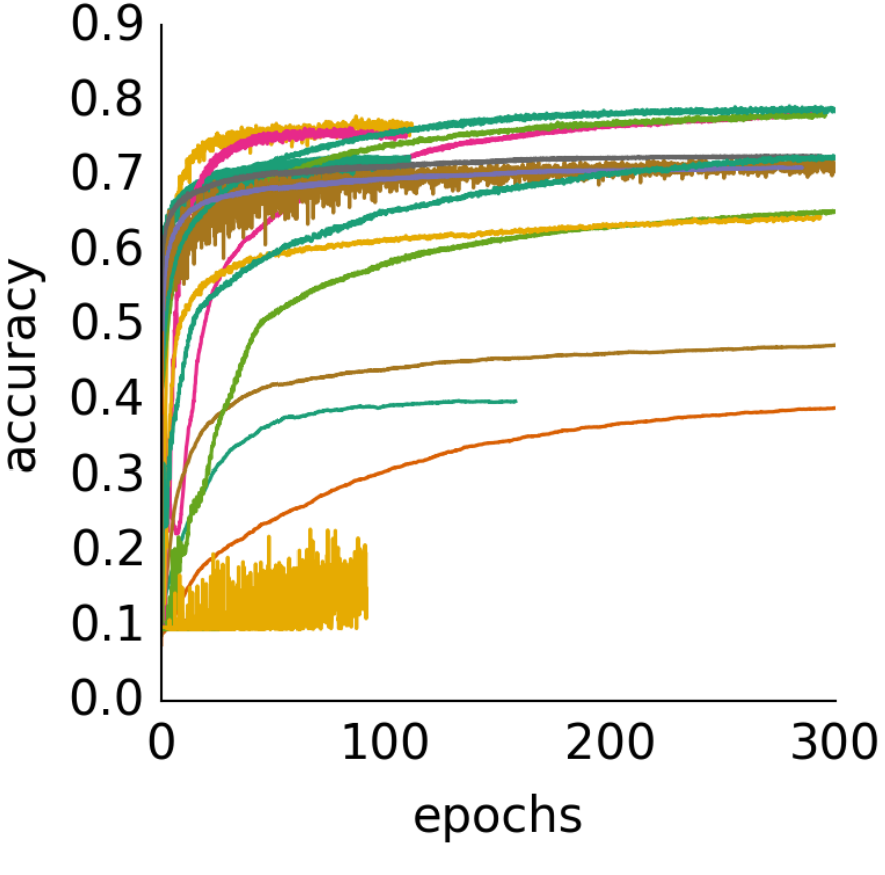
\includegraphics[width=0.4\textwidth]{../w07_hpo_speedup/images/intro/learning_curves.png}

Exemplary learning curves of training deep neural networks\\
Many ML algorithms iteratively optimize a (loss) function

\end{frame}
%-------------------------------------------------
%-------------------------------------------------
\begin{frame}{Stopping poor evaluations early}

\centering
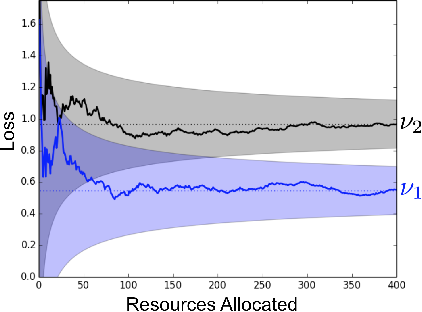
\includegraphics[width=0.5\textwidth]{../w07_hpo_speedup/images/intro/differetiatingConfigurations.png}

Only stop evaluations after they have spent sufficient resources to differentiate between them in terms of quality.

\end{frame}
\fi
\end{document}
